\mode*

\section{Moduler}

\begin{frame}[fragile]
  \begin{lstlisting}[numbers=none,basicstyle=\huge]
import module
  \end{lstlisting}
\end{frame}

\subsection{Hur?}

\begin{frame}[fragile]
  \begin{example}[bad-module.py]
    \lstinputlisting{examples/bad_module.py}
  \end{example}
\end{frame}

\begin{frame}[fragile]
  \begin{example}[test-good-bad.py]
    \lstinputlisting{examples/test_good_bad.py}
  \end{example}
\end{frame}

\begin{frame}[fragile]
  \begin{example}[good-module.py]
    \lstinputlisting{examples/good_module.py}
  \end{example}
\end{frame}

\subsection{Ett gammalt exempel}

\begin{frame}[fragile]
  \begin{example}[input-type.py, del 1]
    \lstinputlisting[linerange=1-13]{examples/input_type.py}
  \end{example}
\end{frame}

\begin{frame}[fragile]
  \begin{example}[input-type.py, del 2]
    \lstinputlisting[firstline=14,firstnumber=14]{examples/input_type.py}
  \end{example}
\end{frame}

\begin{frame}[fragile]
  \begin{example}[Använda modulen]
    \begin{lstlisting}
import input_type

x = input_type(int, "x = ")
print(f"x = {x}")
    \end{lstlisting}
  \end{example}
\end{frame}


\section{PyPI}

\begin{frame}
  
\includegraphics[width=\columnwidth]{figs/pypi.png}
\end{frame}

\begin{frame}
  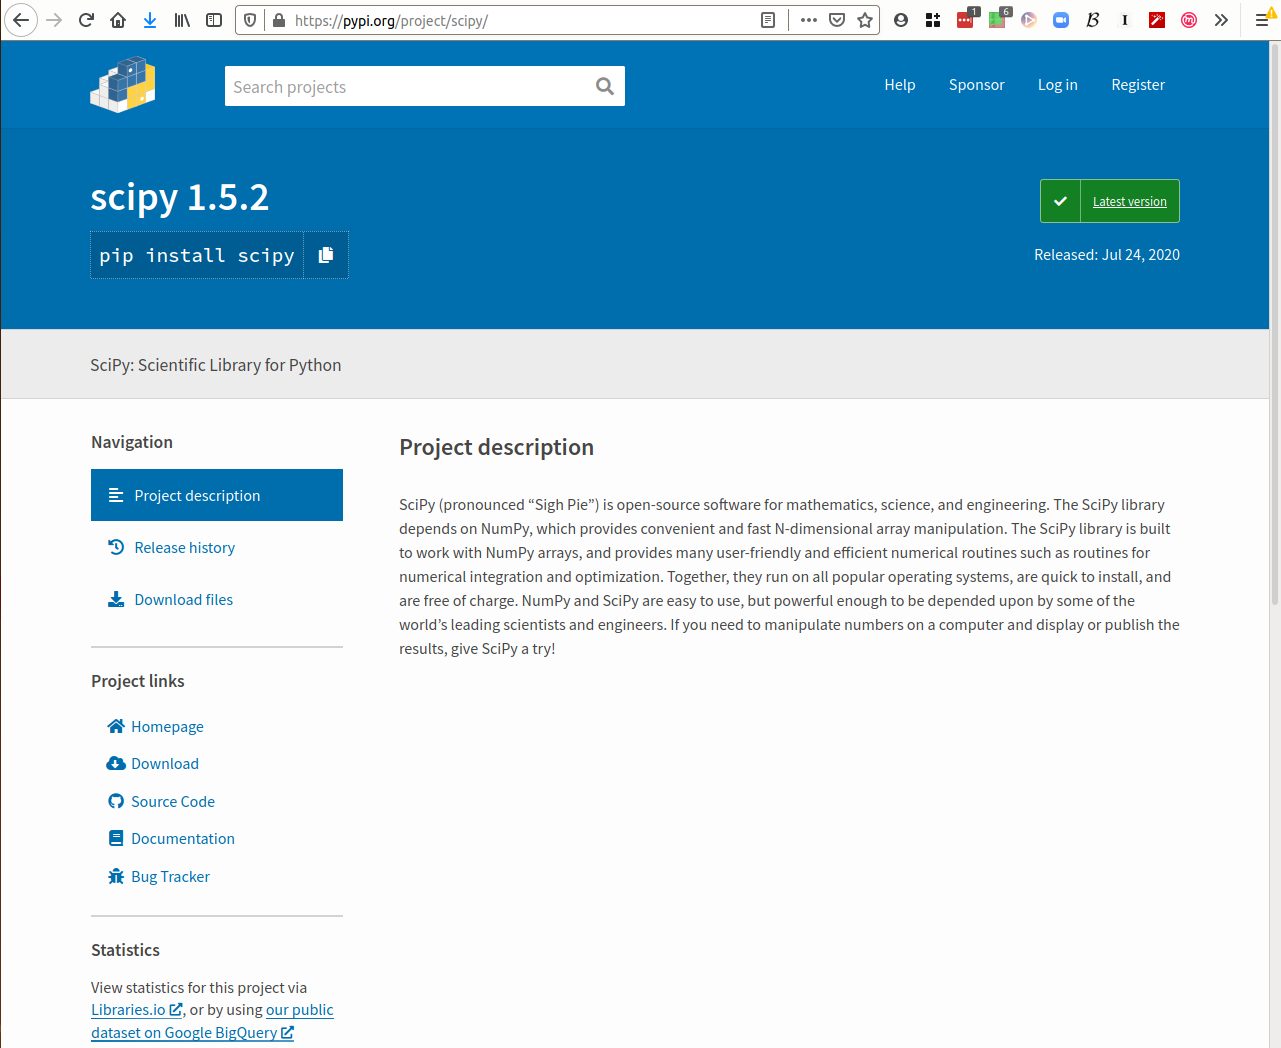
\includegraphics[width=\columnwidth]{figs/pypi-scipy.png}
\end{frame}

\begin{frame}
  
\includegraphics[width=\columnwidth]{figs/pypi-matplotlib.png}
\end{frame}

\begin{frame}[fragile]
  \begin{example}[Installation]
    \begin{lstlisting}[language={},numbers=none]
$ python3 -m pip install numpy scipy matplotlib
    \end{lstlisting}
  \end{example}
\end{frame}

\begin{frame}
  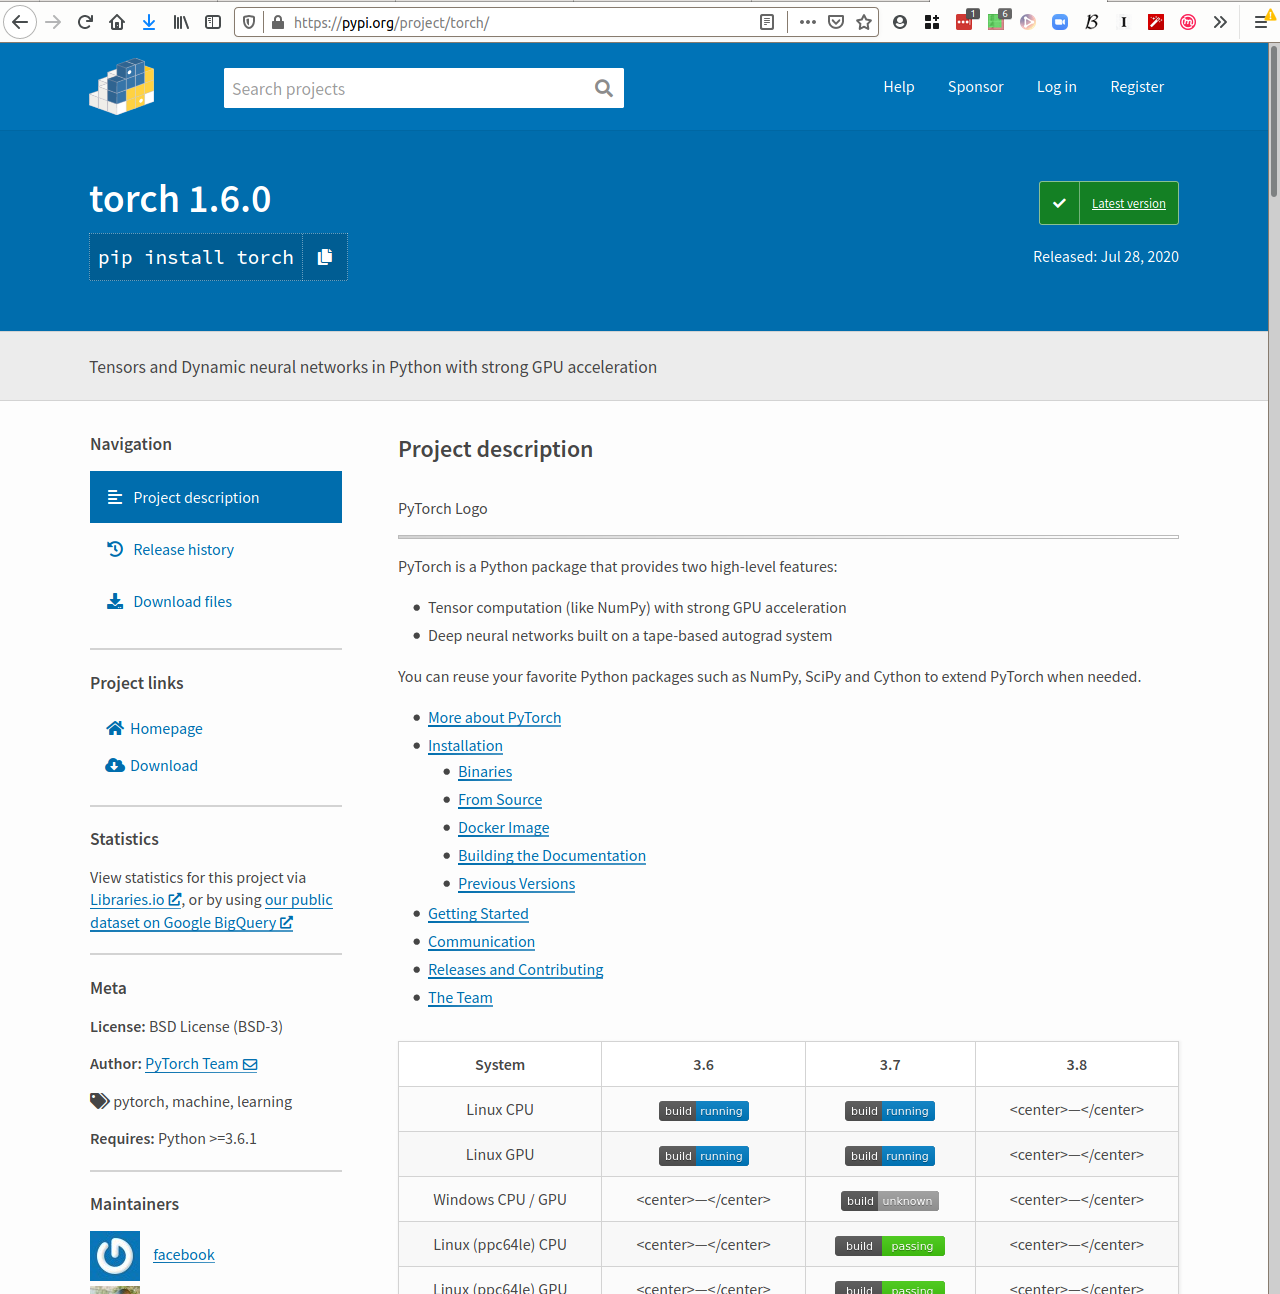
\includegraphics[width=\columnwidth]{figs/pypi-torch.png}
\end{frame}

